\chapter{Non-equilibirum Statistic Physics}

\section{Boltzmann integral ODE}

At the equilibirum state, we have a distribution function, aka a function of the energy that independent from the time
\begin{equation}
  f_0 = f_0(\bm r) = f_0(E)
\end{equation}
which only depends on $r$ and $E$.
\begin{equation}
  f_0 = \frac1{\upe^{\beta E} \pm 1} \xrightarrow{Non-equilibirum}
  f(\bm r, \bm v, t)
\end{equation}
This is the Boltzmann equation for the classical short-term interaction thin gas.
\begin{enumext}
  \item Classical: $\lambda_T \ll |\overline{\delta r}|$,
  $\lambda_T = \frac h{(2\pi mk_BT)^{1/2}}$ is the high-temperature wavelength.
  The gas under the standard state
  ($\qty0\degreeCelsius$, $\qty1{atm}$).
  For the Argon: $n = \qty{2.7e19}{\cm^{-3}}$, $m \approx \qty{6.7e-23}\g$.
  Then
  \[
    \lambda_T = \frac{h}{\sqrt{2\pi mk_BT}} \sim \qty{0.17e-8}\cm, \qq{and}
    \frac{\overline{\delta r}}{\lambda_T} \approxeq 190.
  \]
  \item Thin and Short-term force $\overline{\delta r} \gg d$.
  Most of the gas molecules are free most time.
  Separate the ``hit'' and the ``motion'':
  There is no motion when hitting, or there will be no hitting when moving.
  \[
    \overline{\delta r} \approxeq \qty{3.3e-7}\cm, \quad
    m \sim \qty{6.7e-23}\g, \quad
    \lambda_T = \frac{h}{\sqrt{2\pi mk_BT}} \approxeq \qty{0.17e-8}\cm
  \]
  \item Three-body hitting can be omitted
  
  Taking another simplification
  \begin{enumext}
    \item Omit the structure of molecules, take the rigid-sphere model to instead the Van der Waals force.
    \item There's no relation between the velocities of two hitting molecules.
  \end{enumext}
\end{enumext}
To derive the evolution of $f(\bm r, \bm v, t)$
\[
  f(\bm r, \bm v, t) \d^3\bm r \d^3 \bm v
\]
is the average number of moleculese around the volume unit in the phase
($\bm r$, $\bm v$).
From $t \to t + \d t$
\[
  \frac1{\d t} [f(\bm r, \bm v, t + \d t) - f(\bm r, \bm v, t + \d t)]
  \d^3\bm r \d^3\bm v = \pdv ft \d^3\bm r \d^3\bm v
\]
where $\pdv ft = \ab(\pdv ft)_d + \ab(\pdv ft)_c$: d stands for the drift,
and c stands for the collision.

\subsection{Derivation of the drift term}

Since
\[
  \d f = \ab[f(\bm r + \dot{\bm r} \d t, \bm v + d\bm v, t + \d t)
            -f(\bm r, \bm v, t)] \d t = 0
\]
then,
\[
  \odv ft = \ab(\pdv ft)_d + \sum_i \ab(\dot x_i \pdv f{\dot x_i}
+ \dot v_i \pdv f{v_i}) = 0
\]
So, the drift term
\[
  \ab(\pdv ft)_d = -\bm r \cdot \pdv fr - \bm r \cdot \pdv f{\bm r}
= -\pdv*{\bm rf}{\bm r} - \pdv*{\bm vf}{\bm v}
\]

\subsection{Derivation of the collision term}

To derive the collision term, consider the collision between two particles
\begin{gather*}
  m_1 \bm v_1 + m_2 \bm v_2 = m_1 \bm v_1' + m_2 \bm v_2'\\
  \frac12m_1 v_1^2 + \frac12m_2 v_2^2 = 
  \frac12m_1 v_1'^2 + \frac12m_2 v_2'^2
\end{gather*}
Since at the normal dirction, $v_{1_\bot}' = v_{1_\bot}$.
Then the bound condition
\[
  \bm v_1' - \bm v_1 = \lambda_1 \bm n, \qq{and}
  \bm v_2' - \bm v_2 = \lambda_2 \bm n
\]
For a given $\bm n$, we can solve
\begin{gather*}
  \bm v_1' = \bm v_1 + \frac{2m_2}{m_1 + m_2} [(\bm v_2 - \bm v_1) \cdot \bm n] \bm n\\
  \bm v_2' = \bm v_12 - \frac{2m_1}{m_1 + m_2} [(\bm v_2 - \bm v_1) \cdot \bm n] \bm n
\end{gather*}
Then, we have
\[
  \bm v_2' - \bm v_1' = \bm v_2 - \bm v_1' - 2[(\bm v_2 - \bm v_1) \cdot \bm n] \bm n, \quad
  (\bm v_2' - \bm v_1')^2 = (\bm v_2 - \bm v_1)^2, \quad
  v_{12}'^2 = v_{12}^2.
\]
To calculate $\ab(\pdv ft)_c$
\[
  f_i = f(\bm r, \bm v_i, t), \quad f_i'(\bm r, \bm v_i', t)
\]
$\Delta f_1^{(t)}$ is the collision in the $\d^3\bm r$ space during the $\d t$ time. Then,
\[
  \ab(\pdv{f_1}t)_c \d t \d^3\bm r \d^3\bm r_1
= \Delta f_1^{(+)} - \Delta f_1^{(-)}
\]
When the two molecules collide, if collide with the $m_2$ molecule with the
centre of $\bm r_2$ within the volume unit of $\d^3\bm r_2$, then, the collision
direction will be limited in the cubic angle $\d\Omega$ with the normal vector $\bm n$.

Then, it must be limited in a cylinder with height $v_{12} \cos\theta\d t$ and
with the lower square $r_{12}^2\d\Omega$.
The volume of the cylinder is $r_{12}^2 \d\Omega v_{12} \cos\theta\d t$,
where includes the number of molecules with $\d^3v_{12}$
\[
  (f_2\d^3r_2) r_{12}I^2 \d\Omega v_{12} \cos\theta \d t
\]
Multiply the number of molecules $m$
\[
  (f_1 \d^3\bm r \d^3\bm v_1)(f_2 \d^3r_2) r_{12} \d\Omega v_{12}\cos\theta \d t
\]
equal to the number of collisions between molecules in $\d^3\bm r \d^3\bm v_1$
and molecules in $\d^3\bm r_2$ within the $\d\Omega$ direction during time
$\d t$ is equal to the number of collisions between molecules in
$\d^3\bm r \d^3\bm v_1$ and molecules in $\d^3\bm r_2$ within the domega
direction.

$\delta f_1^{(-)}$ enable the decrease of molecules within $\d^3\bm v_1$:
$(\bm v_1, \bm v_2) \to (\bm v_1', \bm v_2')$
\[
  \delta f_1^{(+)} = \ab[f_1' f_2' \lambda_{12}' \d\Omega' \d^3\bm v_2']
  \d t \d^3\bm r_1 \d^3 \bm v_1'
\]
with $(\bm v_1', \bm v_2', -\bm n) \to (\bm v_1, \bm v_2)$, and the transformation
\[
  \d^3 \bm v_1' \d^3\bm v_2' = \d^3v_1 \d^3\bm v_2
  \begin{vmatrix}
    \pdv{v_1}{v_1'} & \pdv{v_2}{v_1'}\\
    \pdv{v_1}{v_2'} & \pdv{v_2}{v_2'}
  \end{vmatrix}.
\]
Then,
\[
  \ab(\pdv ft)_c \d t \d^3\bm r_1 \d^3\bm v_1 = \Delta f_1^{(+)} - \Delta f_1^{(-)}
  = \int [(f_1'f_2' - f_1f_2) \d^3\bm v_2 \lambda_{12} \d\Omega] \d t \d^3\bm v_1 \d^3\bm v_1
\]
\[
  \pdv ft - \ab(\pdv ft)_d = \ab(\pdv ft)_c
\]
\[
  \pdv ft + \bm v \cdot \ab(\pdv fr) + \bm g \cdot \pdv f{\bm v}
= \int(f_v' f_w' - f_vf_w)  \lambda \d^3 \bm\omega \d\Omega
\]

\section{$H$-theomre, $H$-function and entropy}

The Entropy
\begin{equation}
  S = -\sum_i p_i \ln p_i
\end{equation}
The $H$-function
\begin{equation}
  H = \int f(\bm r, \bm v, t) \ln f(\bm r, \bm v, t) \d^3\bm v \d^3\bm r
\end{equation}
The gas at the equilibirum state
\[
  n = N/V
\]
The Maxwell distribution
\begin{equation}
  f = n\ab(\frac m{2\pi k_BT})^{3/2} \exp\ab(-\frac{mv^2}{2k_BT})
\end{equation}
Then, the $H$-function becomes
\begin{equation}
  H = \int f\ab[\ln n + \frac32\ln\frac m{2\pi k_BT} - \frac{mv^2}{2k_BT}]
      \d^3\bm r \d^3\bm v
\end{equation}
where the integral
\[
  \int f \d^3\bm r \d^3\bm v = n, \quad
  \frac1n\int\frac{mv^2}{2} f\d^3\bm v = \frac32k_BT
\]
The entropy of single-atom ideal gas
\[
  S = Nk_B\ab[\ln\frac VN + \frac32\ln T + \frac52 + \frac32\ln\ab(\frac{2\pi mk_B}{h^2})]
= -k_BH + C
\]
Use the Boltzmann equation to derive the $H$-theorem
\begin{equation}
  \odv HT \leq 0
\end{equation}
The time derivative to $H$
\begin{align*}
  \odv HT & = \int \ab(\pdv ft \ln F + f \cdot \frac1f) \d^3\bm r \d^3\bm v
  = \int (1 + \ln f) \pdv ft \d^3\bm r \d^3\bm v\\
& = -\int (1 + \ln f) \ab(\bm v \cdot \pdv f{\bm r}) \d^3\bm r \d^3\bm v
  -\int (1 + \ln f)(\bm q \cdot \pdv f{\bm v}) \d^3\bm r \d^3\bm v
  -\int (1 + \ln f)(f_1f_2 - f_1'f_2') \d^3\bm v\d^3\bm v'
    \Lambda \d\Omega \d^3\bm r
\end{align*}
The first term
\[
  \nabla \cdot(\bm v f\ln f) = \bm v(1 + \ln f) \pdv f{\bm r}
\]
\[
  \int \d^3\bm r \nabla \cdot (\bm v f \ln f)
= \oiint \bm n \cdot (\bm v f - \ln f) \d\Sigma = 0
\]
The second term $\pdv*{\bm q}{\bm v} = 0$
\[
  \int\pdv*{\bm q f\ln f}{\bm v} \d^3\bm v
= \oiint \d\bm S_v \cdot \bm q f \ln f
\]
when $v \to \infty$, $ f(v)\big|_{v\to\infty} = 0$.
The third term: $1 \leftrightarrow 2$,
\[
  \odv HT = -\int (1 + \ln f_2)(f_1f_2 - f_1'f_2') \d^3\bm v_1 \d^3\bm r_2
  \Lambda \d\omega \d^3\bm r
\]
Combine and then half
\[
  \odv Ht = -\frac12 \int (2 + \ln(f_1f_2)) (f_1f_2 - f_1'f_2') \d(\cdots)
\]
$v_{1,2}' \leftrightarrow v_{1,2}$, we have
\[
  \odv Ht = -\frac12 \int (2 + \ln (f_2'f_1;)) (f_1'f_2' - f_1f_2) \d(\cdots)
= -\frac14 \underbrace{
    \ab(\ln(f_1f_2) - \ln(f_1'f_2^2)) (f_1f_1 - f_1'f_2') \d(\cdots)}_{\geq 0}
\]
Then, $\odv Ht \leq 0$, $\odv St \geq 0$.
When $f_1f_2 = f_1'f_2'$ (Detailed equilibrium condition), they equal to zero.

\section{Application of Boltzmann Equation}

The relaxation time approximation
\begin{equation}
  \ab(\pdv ft)_c = -\frac{f - f^{(0)}}{\tau}
\end{equation}
where $\tau$ is the relaxation time that tends to equilibirum, independent of
$\bm r$. Assum $f$ is also independent of $\bm r$.
Without the external force,
\[
  \pdv ft = -\frac{f - f^{(0)}}{t}
\]
Then, we have
\begin{gather*}
  \frac{\d(f - f^{(0)})}{f - f^{(0)}} = -\frac{\d t}{\tau},\\
  f(\bm v) - f^{(0)}(\bm v) = [f(\bm v, 0) - f^{(0)}(\bm v)] \upe^{-t/\tau}
\end{gather*}
$\tau$ is the time that required by tending to equilibirum.
In the free electon gas,
\[
  f^{(0)}(\bm p) = \frac1{\upe^{(\epsilon(p) - \mu)/k_BT} + 1}
\]
and the Fermi energy $\epsilon(p) = \frac{p^2}{2m}$.

In the unit volume, the average electron number that with in the momentum range
$\d^3\bm p$ is $2\frac{\d^3\bm p}{h^3} f^{(0)}$.

The Boltzmann equation
\[
  \pdv ft + \frac{\bm p}{m} \cdot \pdv f{\bm r} + \bm F \cdot \pdv f{\bm p}
= -\frac{f - f^{(0)}}{\tau}
\]
where $\bm F = -e\bm E$, i.e., the ecurrent is a uniform and eternal
\[
  \pdv ft = 0, \quad \nabla f = 0, -e\bm E \cdot \pdv f{\bm p} = -\frac{f - f^{(0)}}{\tau}
\]
where $f = f^{(0)} + f^{(1) + \cdots}$, and we keep the first order
\[
  e\bm E \cdot \pdv{f^{(0)}}{\bm p} = \frac{f^{(1)}}{\tau} \quad
  f^{(1)} = e\tau\bm E \cdot \bm v \pdv{f^{(0)}}E
\]
Hence,
\[
  f \approxeq f^{(0)} + e\tau \bm E \cdot \bm v \pdv{f^{(0)}}\epsilon
  = f^{(0)}(\epsilon + e\tau\bm E \cdot \bm v)
\]
where
\[
  \pdv{f^{(0)}}{\bm p} = \pdv{f^{(0)}}\epsilon  \pdv\epsilon\beta
= \pdv{f^{(0)}}\epsilon \bm v
\]
The $\bm E$ patt through $\d\bm A$ perpendicularly, hence
\[
  \int J_e \d t \d A = e\int v_x \d t \d A f\frac{2\d^3\bm p}{h^3}
\]
where
\[
  J_e = nev_x = \frac{2\d^3\bm p}{h^3} f ev_x
= 2e\int v_x(\cancel{f^{(0)}} + f^{(1)}) \frac{\d^3\bm p}{h^3}
\]
and we have
\[
  v_p = \frac km, \qq{and} f^{(0)}(v_x) = f^{(0)}(-v_x)
\]
Now, handel $\d^3\bm p$
\[
  \d^3\bm p = p^2\d p \int \d\theta \sin\theta\d\varphi
= 2m\epsilon \d(\sqrt{2m}\sqrt\epsilon) \cdot 4\pi
= \frac{4\pi(2m)^{3/2}}{2} \epsilon^{1/2} \d\epsilon
\]
Substitute it into $J_e$
\[
  J_e = 2eEt \int v_x^2 \pdv{f^{(0)}}\epsilon \frac{\d^3\bm p}{h^3}
= e^2 E\tau, \quad
  \int v_x^2 \pdv{f^{(0)}}\epsilon D(\epsilon) \d\epsilon
\]
where
\[
  D(\epsilon) = 4\pi \frac{(2m)^{3/2}}{h^3} \epsilon^{1/2}
\]
Finally,
\[
  J_e = e^2E\int \tau \frac{v^3}{3} \pdv{f^{(0)}}t D(\epsilon) \d\epsilon
\]
Around $T \sim 0$, $f^{(0)} = \theta(\epsilon - \mu)$. Then,
\[
  J = \frac{2e^2t}{3m} \mu D(\mu) E, \quad
  n = \int_0^\mu D(\epsilon) \d\epsilon = \frac23 \mu D(\mu)
\]
We can use it to calculate the conductivity,
\[
  J_e = \frac{ne^2\tau}{m} E = \sigma E, \qq{where} \sigma = \frac{ne\tau}{m}
\]
The force
\begin{equation}
  \bm F = -e\bm E - \frac ec \bm v \times \bm B
\end{equation}
where $\bm v = (v_x, v_y)$, $v = v_x + \iu v_y$.
The stability
\[
  \pdv ft + \bm v \cdot \nabla f = 0
= -\frac{\bm F}{m} \cdot \pdv f{\bm v} + \ab(\pdv ft)_c
\]
The derivative
\[
  0 = \odv{\braket<v>}t
    = -\frac{eE}{m} + \iu\omega_c \braket<v> - \frac{\braket<v>}{\tau},
  \qq{where}
  \braket<v> = -\frac{eE/m}{1 - \iu\omega_c\tau}
\]
Substitute $E = E_x + \iu E_y$, $\omega_c = \frac{eB}{mc}$,
the current density
\[
  \bm j = \mathbf \sigma \cdot \bm E =
  \begin{pmatrix}
    \sigma_{xx} & \sigma_{xy}\\
    \sigma_{yx} & \sigma_{yy}
  \end{pmatrix}
  \begin{pmatrix}
    E_x \\ E_y
  \end{pmatrix} = j_x + \iu j_y
\]
So, we have the elements of the conductivity matrix
\[
  \sigma_{xx} = \sigma_{yy} = \frac{\sigma_0}{1 + \omega^2\tau^2}, \quad
  \sigma_{xy} = -\sigma_{yx} = -\frac{nce}{B} - \frac{\sigma_{xx}}{\omega_c\tau}
\]
where $\sigma_0 = \frac{ne^2\tau}{m}$.

\section{Fluctuation Phenomenon: Themoral Variables}

\subsection{Regrex System}

The fluctuation of energy
\begin{equation}
  \frac{\sqrt{\braket<(E - \braket<E>)^2>}}{\braket<E>} \sim \frac1{\sqrt N},
  \qq{and} n = \frac NV \qq{finite}
\end{equation}
are all the fluctuations corresponding the microscope variable.

\subsection{Quasi-Themoral Theory (Smoluchowski-Einstein Method)}


The theromal entropy
\begin{equation}
  \bar S = k_B \ln W_{\max} \qq{(theromal probability)}
\end{equation}
where $W_{\max} = \upe^{\bar S/k_B}$.

The differ from equilibirum
\[
  W = \upe^{S/k_B} = W_{\max} \upe^{(S - \bar S)/k_B}
    = W_{\max} \upe^{\Delta S/k_B}
\]
\begin{enumext}
  \item For dependent system, $\Delta E = 0$, $\Delta V = 0$.
  \item For regrex system,
  $\Delta E + \Delta E_e = 0$,
  $\Delta V + \Delta V_e = 0$.
  \begin{align*}
    W_T & = W_{\max} \upe^{(\Delta S + \Delta S_e)/k_B}
  = W_{\max} \upe^{\ab(\Delta S + \frac{\Delta E_e + pV_e}{T})/k_B}\\ &
  = W_{\max} \upe^{(\Delta S T - \Delta E - p\Delta V)/(k_BT)}
  = W_{\max} \upe^{-(\Delta F + p\Delta V)/(k_BT)}
  \end{align*}
\end{enumext}
The free energy
\begin{equation}
  \Delta F = \underbrace{\ab(\pdv FV)_T}_{-p} \delta V
  + \frac12 \underbrace{\ab(\pdv[2]FV)_T}_{-\pdv p/V} (\Delta V)^2
  + \cdots
\end{equation}
Then,
\begin{equation}
  W_T \approxeq W_{\max} \exp\ab[\frac1{2k_BT} \ab(\pdv pV)_T (\Delta V)^2]
\end{equation}
The probability of the quasi-themoral in regrex system
\begin{equation}
  \braket<(\Delta A)^2>
= \frac{\int (\Delta A^2) W \d(\Delta A)}{\int W\d(\Delta A)}
\end{equation}
\begin{example}
  Calculate $\braket<(\Delta V)^2>$.
  \begin{align*}
  & \frac{\int_{-\infty}^\infty (\Delta V)^2
      \exp\ab[\frac1{2k_BT}\ab(\pdv PV)_T(\Delta V)^2] \d(\Delta V)}
    {\text{normalization factor}}\\
= & \frac1{\int \cdots} \int_{-\infty}^\infty (\Delta V)^2
    \frac{k_BT}{(\pdv p/V)_T}
    \frac1{\Delta V} \d\ab\{\exp\ab[\frac1{2k_BT} (\pdv p/V)_T (\Delta V)^2]\}\\
= & \frac1{\int \cdots} \frac{\Delta V(k_BT)}{(\pdv p/V)_T}
    \exp\ab[-\frac1{2k_BT}\ab|\ab(\pdv pV)_T| (\Delta V)^2]
    \bigg|_{-\infty}^\infty - k_BT \ab(\pdv Vp)_T = -k_BT\ab(\pdv Vp)_T
  \end{align*}
  Then, we have
  \[
    \frac{\braket<(\Delta V)^2>}{V^2} = -\frac{k_BT}{V^2} \ab(\pdv Vp)_T
  \]
  If the mass of the system $M = \text{Const}$, i.e., $M = pV$ is fixed. Then,
  \[
    \Delta M = \Delta\rho V + \rho\Delta V = 0 \Rightarrow
    \frac{\Delta\rho}{\rho} = -\frac{\Delta V}{V}, \quad
    \frac{\braket<(\Delta\rho)^2>}{\rho^2} = \frac{\braket<(\Delta V)^2>}{V^2}
  = -k_BT \ab(\pdv Vp)
  \]
  $\rho = N/V$, if $V$ is fixed, then $\Delta \rho \propto \Delta N$.
  \begin{gather*}
    \braket*<\ab(\frac{\Delta N}{N})^2> =
    \braket*<\ab(\frac{\Delta \rho}{\rho})^2> = -\frac{k_BT}{V^2} \ab(\pdv Vp)_T\\
    \Delta\rho = \frac{\Delta N}{V} - \frac{N\Delta V}{V^2}\\
    (\Delta\rho)^2 = \ab(\frac{\Delta N}{V})^2 - \frac{2\Delta N\Delta V}{V^3} + \frac{N^2(\Delta V)^2}{V^4}\\
    \braket<(\Delta \rho)^2> = \braket<\ab(\frac{\Delta N}{V})^2> + \frac{N^2\braket<(\Delta V)^2>}{V^4}\\
    \frac{\braket<(\Delta\rho)^2>}{N^2} =
    \frac{\braket<(\Delta N)^2>}{N^2} + \frac{\braket<(\Delta N)^2>}{N^2}
  = 2\braket<\ab(\frac{\Delta N}{N})^2>
  \end{gather*}
  The critical point
  \[
    \ab(\pdv pV)_T = \ab(\pdv[2]pV)_T = 0
  \]
  Then,
  \[
    \Delta F = -p\Delta V - \frac1{4!} \ab(\pdv[3]pV)_T (\Delta V)^4 + \cdots
  \]
  \[
    W = W_{\max} \exp(-\alpha x^4), \quad x = \Delta V
  \]
  \[
    \braket<(\Delta V)^2>
  = \frac{\int_0^\infty x^2 \upe^{-\alpha x^4} \d x}
      {\int_0^\infty \upe^{-\alpha x^4} \d x}
  = \frac{\Gamma(\frac34)}{\Gamma(\frac14)} \frac1{\sqrt\alpha}
  = 0.338\frac1{\sqrt\alpha}
  \]
\end{example}

\subsection{Vande vars Gas}

\[
  p_c = \frac a{27b^2}, \quad v_c = 3b, \quad T_c = \frac{8a}{27bR}
\]
Substitute them into the ideal gas formula
\[
  \ab(p + \frac a{v^2}) (v - b) = RT, \quad
  p = \frac{3RT}{3V - V_c} - \frac{9RT_cv_c}{8v^2}, \quad
  V = \frac N{N_a} \sigma, \quad N_a = \num{6.02e23}
\]
Then,
\[
  p = \frac{3Nk_BT}{3V - V_c} - \frac{9N k_BT_cV_c}{8V^2}
\]
The derivatives
\begin{gather*}
  \ab(\pdv[3]pV)_T = -\frac{486Nk_BT}{(3V - V_c)^4} + \frac{27Nk_BT_cV_c}{V^5}\\
  \ab(\pdv[3]pV)_{T_c} = -\frac{27Nk_BT_c}{8V_c^4}
\end{gather*}
Finally, we have
\[
  \ab(\frac{\Delta V}V)_c^2 = 0.338\ab[-\frac{V_c^4}{24kT_c}
  \ab(\pdv[3]pV)_c]^{-1/2}
= 0.901/\sqrt N
\]

\begin{example}[The sky is blue (When the air is clean, not frog / haze)]
  The magnitude of the scatter of light
  \[
    I \propto \frac1{\lambda^4} \frac{\braket<(\Delta\rho)^2>}{\rho^2}
  \]
\end{example}

\begin{example}[Liquid]
  \[
    \frac{\braket<I>}{V} \propto
    \frac1{\lambda^4} V \ab[-\frac{V^4}{24k_BT}\ab(\pdv[3]pV)_T]^{1/2}
  \propto \frac1{\sqrt N}
  \]
\end{example}


\section{Fluctuation Phenomenon (Random External Forces, Brown Motions)}

\subsection{Langevin equation}

For particles: $\num{e-5} \sim \qty{e-4}\cm$.
\begin{enumext}
  \item For fixed external forces: Gravity, Buoyancy, Viscous Force.
  \item Random forces: $\qty{e-4}\cm$, liquid molecule density
  $n = \qty{e22}{\cm^{-3}}$, the collisions occur $10^{22-4}/\unit\s$.
  
  For gas: $n \sim \num{e19}$, collision occurs $\qty{e15}{/\s}$.

  Fluctuation forces: the eigen time of collisions
  $\num{e-18} \sim \num{e-15} \unit\s$.
  \[
    m\odv{\bm u}t = \bm F_1 + \bm F_2(t), \quad
    \bm u = \odv{\bm x}t, \quad \bm u = u_x
  \]
  where $F$ is the viscous force: $F_1 = -\alpha u$, $F_2 = x(t)$.
  \[
    m\braket<u> = kT, \quad
    \odv[2]{\braket<x^2>}t + \frac1\tau \odv*{\braket<x^2>}t - \frac{2kT}{m} = 0,\quad
    \tau = \ab(\frac\alpha m)^{-1}
  \]
  Then, the solution
  \[
    \braket<x^2> = \frac{2kT\tau}{m}t + C_1\upe^{-t/\tau} + C_2
  \]
  and substitute the initial condition $t = 0$, $\braket<x^2>$,
  $\odv*{\braket<x^2>}t = 0$. Hence,
  \begin{equation}
    \braket<x^2>
  = \frac{2kT\tau^2}{m} \ab[\frac t\tau - \ab(1 - \upe^{-t/\tau})]
  \end{equation}
  \begin{enumext}
    \item If the observe time $t \ll \tau$,
    \[
      \braket<x^2> = \frac{2kT\tau}{m}, \quad
      \ab(\frac t\tau - (1 - 1 + \frac t\tau - \frac12 \frac{t^2}{\tau^2}))
    = \frac{kT}{m}t^2 = \braket<u^2>t^2
    \]
    \item If $t \gg \tau$, then
    \[
      \braket<x^2> \approxeq \frac{2kT\tau}{m}t
    = \frac{2kT}{\alpha}t = 2Dt \propto t
    \]
  \end{enumext}
\end{enumext}

\subsection{The Diffusion of Brown particles}

Assume $n(x,t)\d x$ is in the range of $(x, x + \d x)$ at time $t$,
introduce $f(x,t) \d x$ for the Brownian particle number of the unit area
perpendicular to $x$-axis:
The probability of a particle at $t = 0$ and located at $x = 0$ to time $t$ is
transformed to $(x, x + \d x)$.
\begin{equation}
  n(x, t+ \tau) = \int_{-\infty}^\infty f(x - x', \tau) n(x', t) \d x'
= \int_{-\infty}^\infty f(\xi, \tau) n(x - \xi, t) \d\xi
\end{equation}
where
\[
  \int_{-\infty}^\infty \d x f(x, \tau) = 1, \qq{and}
  f(x, \tau) = f(-x, \tau)
\]
For small $\tau$
\begin{equation}
  n(x, t + \tau) = n(x, t) + \tau\pdv nt + \frac12 \tau^2 \pdv[2]nt + \cdots
\end{equation}
For small $\xi$
\begin{equation}
  n(x - \xi, t) = n(x, t) - \xi \pdv nx + \frac12 \xi^2 \pdv[2]nt + \cdots
\end{equation}
Assume when $\xi$ is large, $n(x - \xi, t)$ is small. Then,
\begin{equation}
  n(x, t + \tau) \approxeq n(x, t) + \tau \pdv nt
+ \frac12\tau^2 \pdv[2]nt + \cdots
= \int_{-infty}^\infty \d \xi f(\xi, \tau)
  \ab(n(x,t) - \xi\pdv nx + \frac12 \xi^2 \pdv[2]nx + \xi^3\xi^4),
\end{equation}
where $\pdv nt = D\pdv[2]nx, \quad D = \frac{\braket<\xi^2>}{2\tau}$.
\begin{gather}
  \pdv*{n(x, t + t')}{t'} - D\pdv*[2]{n(x, t + t')}x = 0\\
  \int_{-infty}^\infty \ab[\pdv*{f(x - x')}{t'} - D\pdv*[2]{f(x -x ', t')}x]
    n(x', t) \d x' = 0
\end{gather}
So, the kernel
\[
  \pdv{f(\xi, t)}t - D\pdv*[2]{f(\xi, t)}\xi = 0.
\]

\subsection{Time correlation in Brown motion}

\[
  u(t) = g(t) \upe^{-t/\tau}
\]
where
\[
  \odv[fun]{g\upe^{-t/\tau}}t = -\frac{g(t)\upe^{-t/\tau}}\tau
+ \frac{\chi(t)}{m}
\]
Then, we obtain the ODE
\[
  \odv{g(t)}t = \upe^{t/\tau} \frac{\chi(t)}{m} A(t)
\]
the solution
\begin{gather}
  [g(t) - g(0)] \upe^{-t/\tau}
= \upe^{-t/\tau} \int_0^t \upe^{t'/\tau} A(t') \d t'\\
  u(t) = u(0) \upe^{-t/\tau}
       + \upe^{-t/\tau} \int_0^t \upe^{t'/\tau} A(t') \d t'\\
  u^2(t) = u^2(0) + 2u(0)\upe^{-2t/\tau} \int_0^t \upe^{t'/\tau} A(t') \d t'
       + \upe^{2t/\tau} \int_0^t \d t \d t'' \upe^{(t'+t'')/\tau} A(t') A(t'')
\end{gather}
The correlation function determines the expectation value
\begin{equation}
  \braket<u^2(t)> = u^2(0)\upe^{-t/\tau}
+ \upe^{-2t/\tau} \int_0^t \d t' \d t'' \upe^{(t'+t'')/\tau}
  \braket<A(t') A(t'')>
\end{equation}
Take the rotation
\begin{equation}
  \upe^{(t'+t'')} \braket<A(t')A(t'')> \equiv \upe^{\sqrt2 \tilde t/\tau} C(s)
= \int_0^{t/\sqrt2} \d\tilde t \upe^{\sqrt2\tilde t/\tau}
  \int_{-\tilde t}^{\tilde t} C(s) \d x
= + \int_{t/\sqrt2}^{\sqrt2t} \d\tilde t \upe^{\sqrt2\tilde t/\tau}
    \int_{-\sqrt2t+\tilde t}^{\sqrt2t-\tilde t} C(s) \d s
\end{equation}
where $\d t' \d t'' = \d\tilde t\d s$.
\begin{paracol}{2}
  \[
    I = \int \d t' \d t'' \upe^{\sqrt2\tilde t/\tau} C(s)
  \]
  \switchcolumn \centering
  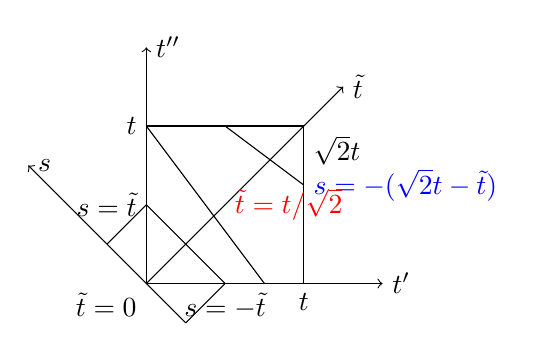
\begin{tikzpicture}
    \draw [->] (0,0) node [below left] {$\tilde t = 0$} -- (3,0)
     node [right] {$t'$};
    \draw [->] (0,0) -- (0,3) node [right] {$t''$};
    \draw [->] (0,0) -- (2.5,2.5) node [right] {$\tilde t$};
    \draw [->] (.5,-.5) -- (-1.5,1.5) node [right] {$s$};
    \draw (0,0) rectangle (2,2) node [below right] {$\sqrt2t$};
    \node [left] at (0,2) {$t$} node [below] at (2,0) {$t$};
    \draw (-.5,.5) -- (0,1) node [left] {$s = \tilde t$} --
          (1,0) node [below] {$s = -\tilde t$} -- (.5,-.5);
    \draw (0,2) -- (1.5,0) (1,2) -- (2,1.25)
     node [blue, right] {$s = -(\sqrt2t - \tilde t)$};
    \node [red, right] at (1,1) {$\tilde t = t/\sqrt2$};
  \end{tikzpicture}
\end{paracol}

Brownian motion $C(s)$ Markov process
\[
  C(s) = C(\delta s), \quad
  I = \frac{Ct}{\Omega} \int_0^{\sqrt2t}
      \d\tilde t \frac{\sqrt2}{2} \upe^{\sqrt2 \tilde t/\tau}
    = C\frac t{\sqrt2}(\upe^{\iu t/\tau} - 1)
\]
Then,
\[
  \braket<u^2(t)> = u^2(0) \upe^{-2t/\tau}
+ C\frac{\tau}{\sqrt2}(1 - \upe^{-2t/\tau})
\]
For $t \to \infty$, $\braket<u^2(\infty)> = kT/m$,
$C = \frac{\sqrt2kT}{m\tau}$,
\[
  \braket<u^2(t)> = u^2(0) \upe^{-2t/\tau} + \frac{kT}{m}(1 - \upe^{-2t/\tau})
\]

\subsection{Fluctuation-Usage Theorem}

The relation between the fluctuation of time and usage for Brownian,
$\tau = \ab(\frac\alpha m)^{-1}$, so
\[
  \alpha = \frac m\tau = \frac{m^2}{\alpha kT}C
= \frac{m^2}{\alpha kT} \int_{-\infty}^\infty \d t\braket<\delta(t)>
= \frac{m^2}{\alpha kT} \int_{-\infty}^\infty \d t \braket<A(0)A(t)>
= \frac{m^2}{\alpha kT} \int_{-\infty}^\infty \d s \braket<A(t + s)A(t)>
\]
We can also prove the distribution coefficient
\begin{equation}
  D = \frac{kT}{\alpha}
= \frac12 \int_{-\infty}^\infty \d u\braket<u(t) u(t + s)>
\end{equation}

\subsection{The themoral conductance noice and the fluctuations in voltage}

In RL circuit, the KVL equation
\[
  L \odv{I(t)}t = -RI(t) + V(t)
\]
where $V_\text{ext} = 0$, $\braket<I(t)> = 0$, $\braket<V(t)> = 0$.
The form of Brown motation
\begin{align}
  I(t) & \leftrightarrow u(t),\\
  L & \leftrightarrow m,\\
  R & \leftrightarrow \alpha,\\
  V(t) & \leftrightarrow \chi(t)
\end{align}
Taking the Foruier transformation
\[
  \tilde V(\omega)
= \frac1{2\pi} \int_{-infty}^\infty V(t) \upe^{-\iu\omega t} \d t
\]
and
\[
  \braket<V(t) V(t + \delta)> = C\delta(s)
\]
\[
  \frac1{4\pi^2} \int \d\omega \d\omega'
  \braket<\tilde V(\omega) \tilde V(\omega')>
  \upe^{\iu\omega t + \iu\omega'(t+s)}
= C\delta(s)
= C\frac1{2\pi} \int \d\omega' \upe^{\iu\omega's}
\]
Assume
\begin{multline}
  \braket<\tilde V(\omega) \tilde V(\omega^2)> 
  = \braket<|\tilde V(\omega)|^2> \delta(\omega + \omega')
  = \frac1{4\pi^2} \int \d\omega \d\omega' \braket<|\hat V(\omega)|^2>
    \upe^{\iu\omega t + \iu\omega(t+s)} \delta(\omega + \omega')\\
  = \frac1{4\pi^2} \int \d\omega'
  \underset{2\pi C \to \text{Independent from $\omega$}}
    {\braket<|\tilde V(\omega')|^2>} \upe^{-\iu\omega's}
\end{multline}
The fluctuation of voltage
\[
  \braket<V^2> = \braket<V^2(t)>
= K(0) = \int_{-\infty}^\infty \tilde K(\omega) \d\omega
= \int_{-\infty}^\infty 4\pi \tilde K(\nu) \d \nu
\]
where $\nu = 2\pi\omega$ and
\begin{enumext}[columns = 2]
  \item $S(\nu) = 4k_BTR \propto T$: Themoral noise
  \item $S(\nu) = 4k_BTR \propto R$: Superconduct: no noise.
  \item $\braket<I^2> \neq 0$
  \item $S(\nu)$ is independent from $\nu$: white noise.
\end{enumext}

\subsection{Shot noise}

\begin{enumext}
  \item The shot of electrons is random
  \item The time between electrons released and arrive at the positive point is
  short, equivalent to a sudden current.
\end{enumext}
If $n(\tau)$ is the number of released electrons in unit time around
time $\tau$, then the current $j(t - \tau)$ at time $\tau$ raised from the
released electrons will getweaker until $0$ when $t - \tau$ is large.
\[
  I(t) = \int_{-\infty}^\infty \d\tau n(\tau) \iu(t - \tau)
\]
and the average
\[
  \braket<I(t)> = \int_{-\infty}^\infty \d\tau \braket<n> \iu(t - \tau)
= \braket<n> \int_{-\infty}^\infty \iu(t - \tau) \d \tau = \braket<n> e
\]
The fluctuation
\[
  \Delta I = I(t) - \braket<I>
= \int_{-\infty}^\infty \d t[n(\tau) - \braket<n>] \iu(t - \tau) \d t
\]
and the square
\[
  \braket<(\Delta I)^2> = \int \d\tau \d\tau'
    \braket<\Delta n(\tau) \Delta n(\tau')> \iu(t - \tau) \iu(t - \tau')
\]
For shot noise,
\begin{gather*}
  \braket<\Delta n(\tau) \Delta n(\tau')> \propto \delta(\tau - \tau'),\\
  \braket<(\Delta I)^2> = \braket<n> \int_{-\infty}^\infty |n(\tau)|^2 \d\tau
= \braket<n> 4\pi \int_0^\infty |S(\omega)|^2 \d\omega
\approxeq 4\pi\braket<n> |S(\omega)|^2 \Delta \omega
\end{gather*}
For a scaler, $S(\omega) = \tau$ only at a given frequency.

If $\omega t \ll 1$, $\upe^{-\iu\omega t} \approx 0$.
\[
  S(\omega) \approxeq \frac1{2\pi} \int_{-\infty}^\infty i(t) \d t = \frac e{2\pi}
\]
Then, we can measure the charge $e^*$ of a quasi-particle.
\[
  \braket<(\Delta I)^2> = 2\braket<n> e^2 \Delta \nu
= 2e^* \braket<I> \Delta \nu*
\]
In 1981: Fractional Quantum Hall Effect $\nu = \frac13$, $e^* = \frac e3$.

\section{Main Equation \& Fock-Planck Equation}

\subsection{Master equation}

\paragraph{Markov Process}

The probability at time $t$ is only related to the former time of the nearest
neighbor state.

Denote $x(t)$ a random variable $(u(t), I(t), \cdots)$.
\begin{enumext}
  \item $P_1(x_1,t_1)$ denotes the probability of the value of $x$ is $x_1$
  at $t_1$.
  \item $P_2(x_1,t_1;x_2,t_2)$ denotes both the value of $x$ is $x_1$ at $t_1$
  and the value of $x$ is $x_2$ at $t_2$, is so-called the united probability.
  \item Similarly for $P_n(x_1,t_1;\cdots;x_n,t_n)$.
  \item $P_{1/1}(x_1,t_1|x_2,t_2)$ is for a given $x$, when its
  value is $x_1$ at time $t_1$, the probability of the value of $x$ is $x_2$
  at $t_2$ (Conditional probability).
\end{enumext}
They satisfy the following identities
\begin{enumext}
  \item $\int P_1(x_1,t_1)\d x_1 = 1$.
  \item $\int P_n(x_1,t_1,\cdots,x_n,t_n) \d x_n
  = P_{n-1}(x_1,t_1,\cdots,x_n,t_n)$.
  \item WHen the system is stable,
  $P_n(x_1,t_1;\cdots,x_n,t_n) = P_n(x_1,t_1+\tau;\cdots,x_n,t_n+\tau)$
  is independent from time.
  \item $P_1(x_1,t_1)P_{1/1}(x_1,t_1|x_2,t_2) = P_2(x_1,t_1;x_2,t_2)$.
  \item $\int P_{1/1}(x_1t_1|x_2t_2)\d x_2 = 1$.
\end{enumext}
In quantum mechanics,
\[
  P_1(x_1,t_1) = |\psi_1(x_1,t_1)|^2, \quad
  P_1(x_1,t_1|x_2,t_2) = |U(x_2,t_2;x_1,t_1)|^2
\]
The latter one denotes the jump probability of
$\ket|\psi_1(x_1,t_1)> \to \ket|\psi_2(x_2,t_2)>$.
\[
  P_{n-1/1}(x_1t_1\cdots x_{n-1}t_{n-1}|x_n,t_n)
= P_{1/1}(x_{n-1}t_{n-1}|x_n,t_n)
\]
\begin{example}
  \begin{multline*}
    P_3(x_1,t_1;x_2,t_2;x_3,t_3)
  = P_2(x_1t_1;x_2t_2) P_{2/1}(x_1t_1;x_2t_2|x_3t_3)\\
  = P_1(x_1t_1) P_{1/1}(x_1t_1;x_2t_2) P_{1/1}(x_2t_2|x_3t_3)
  \end{multline*}
  Integral on both sides by $\d x_2$
  \[
    P_2(x_1t_1;x_3t_2) = P_1(x_1t_1) \quad
    \int \d x_2 P_{1/1}(x_1t_1;x_2t_2) P_{1/1}(x_2t_2;x_3t_3).
  \]
  Div $P_1(x_1,t_2)$ on both sides
  \begin{equation}
    P(x_1t_1;x_3t_3) = \int \d x_2 P(x_1t_2;x_2t_2) P(x_2t_2;x_3t_3)
  \end{equation}
  We obtain the SCK equation.
  Take $t_2 = t + \tau$, $t_1 = t$
  \[
    P(x_2,t + \tau) = \int P(x,t) P(xt|x_2,t + \tau) \d x,
  \]
  The derivatives
  \[
    \pdv{P(x,t)}t = \lim_{\tau\to0} \frac{P(x,t + \tau) - P(x,t)}{\tau},\quad
    \pdv{P(x_2,t)}t = \lim_{\tau\to0} \frac1\tau
      \int P(xt)[P(x,t|x_2,t + \tau) - P(x,t|x_2t)]
  \]
  If $\tau = 0$
  \[
    P(x_2,t) = \int P(xt) P(xt|x_2t) \d x, \quad
    P(xt|x't) = \delta(x - x')
  \]
\end{example}
Denote $W(x_1,x_2)$ is the jump probability density of the value of $x$ changes
from $x_1$ to $x_2$ in unit time during the time interval $t \to t + \tau$,
then $\tau\int W(x_1,x)\d x$ is the total probability of the value $x_1 \to x$
in time interval $\tau$, then $[1 - \tau\int W(x_1,x)\d x]$ is the probability
that the jump will not occurs, if $\delta(x_1 - x_2)$ is multiplied, then  it is
the probability tha keep $x_1 = x_2$ and not other values of $x$.
\[
  P(x_1t|x_2t+\tau) = [1 - \tau\int W(x_1,x)\d x] \delta(x_1 - x_2)
  + W(x_1, x_2)\tau
\]
Take the time derivative
\begin{multline*}
  \pdv{x_0,t}{t} = \frac1\tau\bigg[
      \cancel{\int P(x_1,t)\delta(x_1 - x_2) \d x_1}
    - \int P(x_1,t)\tau \int W(x_1,x)\d x \delta(x_1 - x_2)\d x_1\\
    + \tau \int P(x_1,t)W(x,x_2)
    - \cancel{\int P(x_1,t)\delta(x_1 - x_2) \d x_1}\bigg]
\end{multline*}
we obtain the Master equation
\[
  \pdv{P(x_2,t)}t = \int [W(x_1,x_2)P(x_1,t) - P(x_2,t) W(x_2,x_1)]\d x
\]
\begin{example}
  For a lonely system, its density matrix
  \[
    \rho(t) = \sum_i w_i(t) \ketbra|i><i|
  \]
  and the Hamiltonian
  \[
    H = H_0 + V, \quad H_0\ket|i> = E_i\ket|i>.
  \]
  $U^*(\tau)$ is time evolution operator
  \[
    \rho(t + \tau) = \sum_i w_i(t) U(\tau) \ketbra|i><i| U^\dagger(\tau)
  = \sum_{i,j,k} w_i \ket|j>\braket<j|U(t)|i>\braket<i|U^\dagger|k>\bra<k|
  = \sum_i \sum_{j,k} w_i(t) \ketbra|j><k| U_{ji}(\tau) U_{ki}^*(\tau)
  \]
  Take random phase approximation (RPA)
  \[
    \rho(t + \tau) \approxeq \sum_i \sum_j w_i(t)
    \ketbra|j><j| U_{ji}(t) U_{ji}^*(\tau)
  = \sum_j w_j (t + \tau) \ketbra|j><j|
  \]
  That is
  \[
    w_{j}(t + \tau) = \sum_i w_i(t) |U_{ji}(t)|^2, \quad
    w_j(t + \tau) - w_j(t) = \sum_i (w_i(t) - w_j(t))|U_{ji}(\tau)|^2,
  \]
  where $i = j$ canceled. $|U_{ji}|_{j\neq i}^2$.
  \[
    |U|_{ji}^2 = \frac1{\hbar^2}
      \ab(\frac{\sin(w_{ij}\tau/2)}{w_{ij}/2})^2 |\braket<j|V|i>|^2
    \approxeq \tau \frac{2\pi}{\hbar} \delta(E_i - E_j) |\braket<j|V|i>|^2
  \]
  The derivative
  \[
    \odv{w_i(t)}t = \frac{w_i(t + \tau) - w_i(t)}{\tau}\bigg|_{\tau\to0}
  = \sum_i (w_i(t) - w_j(t))
    \frac{2\pi}{\hbar} \delta(E_i - E_j) |\braket<j|V|i>|^2
  \]
  where $\tau = (E_i - E_j)/\hbar$,
  $\sum_i$ is the sum of all the quantum states.
  Take $\sum_i \to \sum_{E_i,F_i}$,
  then
  \[
    \sum_{E_i} \to \int \d E_i n(E_i),
  \]
  $n(E_i)$ denotes the DOE.
  \[
    \odv{W_{E_iF_i}(t)}t = \sum_{F_i} (W_{E_jF_i} - W_{E_jF_j})
      \ab(\frac{2\pi}{\hbar} n(E_i)|\braket<E_jF_j|V|E_jF_j>|^2 P_{E_j}(E_jF_j))
  \]
\end{example}

\subsection{Forkker-Planck equation}

$x$ can be continuous, $w(x,x')$ will get weaker quickly as the increase
of $|x - x'|$. We can deonote $\xi = x - x'$ as a small variable, then
\[
  W(x',x) = W\ab(\frac{x' + x}{2}, x' - x) \approxeq W(x', -\xi)
\]
Take the approximation to the main equation
\[
  \pdv{P(x,t)}t = \int [w(x',x) P(x',t) - W(x,x') P(x,t)] \d x'
= \int [w(x - \xi, \xi) P(x - \xi, t) - W(x, -\xi) P(x, t)] \d \xi
\]
Expand it
\[
  W(x - \xi,\xi) P(x - \xi,t) = W(x,\xi) P(x,t) - \xi\pdv*{w(x,\xi) P(x,t)}x
+ \frac12\xi^2 \pdv*[2]{[w(x,\xi)P(x,t)]}\xi + \cdots
\]
Substitute the expansion back
\[
  \pdv{P(x,t)}t = \cancel{\int w(x,\xi) P(x,t) \d \xi}
- \int \xi \pdv*{[w(x,\xi)P(x,t)]}x
+ \frac12 \int \xi^2 \pdv*[2]{[w(x,\xi) P(x,t)]}x \d \xi - \cancel{\cdots}
\]
Rearrange
\begin{equation}
  \pdv{P(x,t)}t + \pdv*{[\alpha_1(x) P(x,t)]}x
= \frac12 \pdv*[2]{\alpha_2(x)P(x,t)}x
= \int \xi^n w(x,\xi) \d\xi
\end{equation}
$n$-th matrix. Forkker-Planck equation.
If $\alpha_1(x) = 0$, $\alpha_2(x) = \text{Const}$, then F-P equation is
equivalent to Browian motion equation.